\documentclass[12pt]{article}
\usepackage{xeCJK}
\usepackage{tikz}
\usetikzlibrary{automata, positioning, shapes.geometric}
\usepackage{amsmath, amssymb}
\usepackage{geometry}
\usepackage{fancyhdr}
\usepackage{graphicx}
\usepackage{hyperref}
\usepackage{bm}
\usepackage{cite}
\usepackage{booktabs}   % 漂亮的横线
\usepackage{tabularx}   % 自动伸缩列宽
\usepackage[normalem]{ulem}

\geometry{a4paper,left=32mm,right=32mm,top=25mm,bottom=25mm}
\setCJKmainfont{SimSun}

\title{玩家年龄是否对其游戏表现有意义?\\——以舞萌 \texttt{maimaiDX} 为例}
\author{\textbf{inkCake} | \textbf{舞萌大学 } 数学与统计学院}
\date{\today}

\begin{document}
	\maketitle
	
\section*{摘要}
本文以 SEGA 音乐街机游戏舞萌 DX 为研究场景,采用在线问卷与机台数据结合的方式,收集了 276 份有效样本,以简单随机抽样代表约 50 万活跃玩家总体,在 95\% 置信水平下总体比率估计误差约为 ±6\%。通过派生游玩时长、总游玩次数、起步年龄等核心变量,综合使用描述统计、相关分析、分段非线性可视化与多元 OLS 回归,对“年龄天赋”在玩家表现中的作用进行了量化。结果显示:练习量是决定 Rating 的首要因素,游玩次数仍旧是DX Rating的主要影响成分;控制练习量后,起步年龄与当前年龄对 Rating 均呈显著负向影响,早入坑者的练习收益更高;游玩 1–2 年是表现提升最快的时期,之后呈指数饱和趋势;玩家对“天赋”重要性的主观认知与实际评分差异不显著。综合来看,“年龄天赋”在音乐游戏表现中确实存在,但作用远小于练习投入,总投入与早起步的交互是达到高水平的关键驱动。

	
	\vspace{1em}
	\noindent\textbf{关键词:} 音乐游戏;舞萌 DX;年龄天赋;简单随机抽样;回归分析
	
	
	\newpage
%==================================================
% 第 1 章 研究背景与目的
%==================================================
\section{研究背景与目的}

\subsection{音乐游戏概述}

音乐游戏(rhythm game)起源于 1990 年代日本街机文化,以“节奏精准度”作为核心评分机制。玩家需在伴奏节拍提示下,通过\texttt{按键、触屏或体感}等方式完成预设操作。\texttt{maimai DX} 由 SEGA 于 2012 年推出,采用环形触摸屏配合八键实体按键,兼具“音符密度高、判定严格”与“社交排行榜”特色,现已覆盖亚洲与北美多地。\textbf{舞萌 DX}(中国大陆官方名称)首发于 2019 年,截至 2024 年底共铺设约 2\,700 台机台,注册玩家逾 200 万,其中活跃玩家(近 30~天登录并上传成绩者)约 50 万。

\subsection{国内外研究现状}

\textbf{音乐节奏与音游领域}:早期节奏训练可显著提升感觉—运动同步能力。Watanabe \emph{et~al.}\,(2007) 发现,6–10 岁开始接受节拍训练的受试者在成人阶段保持更低的同步误差;类似结果亦见于 Bailey \& Penhune\,(2013) 对音乐学院学生的纵向研究,后者指出起步年龄每提前一年,节奏一致性可提高约 0.2 个标准差\cite{Watanabe2007,Bailey2013}。

\textbf{电子竞技与动作类视频游戏领域}:大规模实证表明表现与年龄呈倒“U”形。Thompson \emph{et~al.}\,(2014) 追踪 3\,305 名《星际争霸》职业选手的实时操作记录,报告平均反应时在 24 岁后以每年 2.5~ms 的速度下降\cite{Thompson2014}。该结论与 FPS、MOBA 等竞技游戏的职业生涯曲线一致,提示 20 岁出头可能是高反应要求项目的峰值年龄段。

\textbf{体育技能习得与练习效应}:经典“1 万小时定律”指出刻意练习是取得专家表现的关键\cite{Ericsson1993},但更大样本荟萃分析显示,刻意练习仅能解释 18–26\% 的成绩方差\cite{Macnamara2014}。针对奥运项目的回顾研究亦指出,过早专业化并非通向顶尖表现的必要条件,部分运动员在青春期后才转项成功\cite{Gullich2017,Vaeyens2009}。

\noindent\emph{综上},年龄确实影响高水平表现,但效应大小与项目需求、练习强度及个体差异交互作用。本研究通过控制练习量(游玩次数与时长)与起步年龄,量化“年龄天赋”在音乐游戏场景中的独立贡献。

\subsection{研究目的与研究问题}

\begin{enumerate}
	\item \textbf{描述现状:} 以 276 份样本估计国内舞萌 DX 玩家年龄、练习量与成绩分布。
	\item \textbf{检验假说:} 在控制\emph{总游玩次数}与\emph{练习时长}后,\emph{起步年龄}是否仍对最终评分(\texttt{rating}) 有显著影响?
	\item \textbf{量化效应:} 计算年龄相关变量的标准化系数、解释力增量 $\Delta R^2$ 与随机森林特征重要度,衡量“年龄天赋”的贡献度。
	\item \textbf{实践意义:} 为音游赛事分级、曲目推荐与青少年玩家训练方案提供数据支撑。
\end{enumerate}

%==================================================
% 第 2 章 样本与数据来源
%==================================================
\section{样本与数据来源}

\subsection{问卷设计}

本研究核心数据来自自行编制的线上问卷,遵循\emph{最小必要信息}原则以降低填答负担。问卷共 7 个封闭 / 半开放问题(见表~\ref{tab:items}),变量名称与后续实证模型一一对应。

\begin{table}[htbp]
	\centering
	\caption{问卷条目与变量映射}\label{tab:items}
	\begin{tabularx}{\textwidth}{@{} l X @{}}
		\toprule
		\textbf{变量} & \textbf{条目内容} \\
		\midrule
		\texttt{player\_rating} &
		您的最高 \textit{Rating}(默认填写当前 DX 版本;若近期未游玩亦可填历史峰值) \\[2pt]
		\texttt{Question1} &
		您认为“年龄天赋”是否存在?选项:是;否;存在,但不重要 \\[2pt]
		\texttt{birthday} &
		请选择出生日期(年月日) \\[2pt]
		\texttt{Question2} &
		您觉得自己\uline{进步最快}的一年是几岁? \\[2pt]
		\texttt{play\_time\_month} &
		您认真游玩的时长(\emph{入坑时间},单位:月),定义为开始为推分或社交目的而系统练习的时间 \\[2pt]
		\texttt{play\_count} &
		当前累计 PC 数(游玩次数,1\,PC $\approx$ 3–4 首曲目) \\[2pt]
		\texttt{Question3} &
		我还有话想说(对问卷、游戏体验或本研究的任何补充意见,开放文本) \\
		\bottomrule
	\end{tabularx}
\end{table}

为避免“问卷疲劳”与查阅成本过高,仅保留与研究假设直接相关的核心变量。诸如谱面偏好、游玩频率、详细游玩历史等信息虽有潜在价值,但易降低填答意愿,故本次调查暂未纳入。



\subsection{总体与抽样框}

根据运营方公开数据,2024 年底中国大陆机台总数 $N_{\text{machines}}=2{,}700$ 台;若假设各机台月活跃人数均衡,则活跃玩家总体约 $N_{\text{players}}\approx500{,}000$。本研究在QQ空间与QQ群随机投放问卷链接,采用\emph{简单随机抽样}收回问卷 288 份,剔除异常后有效样本 $n=276$。

\paragraph{抽样精度与置信区间}
本研究共回收有效问卷 $n=276$ 份,针对活跃玩家总体 $N\approx500\,000$,采用简单随机抽样。  
以 95\% 置信水平($z_{0.975}=1.96$),最大标准误发生在 $p=0.5$ 时,此时抽样误差(边际误差)为:
\[
\mathrm{ME}
= z_{0.975} \sqrt{\frac{p(1-p)}{n}}
\approx 1.96 \times \sqrt{\frac{0.5 \times 0.5}{276}}
\approx 0.059 \;(\pm 5.9\%)
\]
即对总体比率型指标的估计误差约为 $\pm6\%$。若以 90\% 置信水平($z_{0.95}=1.645$),误差可缩小至约 $\pm5\%$。  
该精度足以支持对单因素效应(年龄)的可靠推断。

\subsection{变量说明}

\begin{itemize}
	\item \textbf{评分指标:} \texttt{DX Rating}(0--16588;官方计算基于最近最佳 50 首成绩加权)。
	\item \textbf{人口学变量:} 当前年龄、首次游玩年龄(起步年龄)。
	\item \textbf{练习量变量:} 累计游玩时长(\texttt{play\_time}),总游玩次数(\texttt{play\_count})。
	\item \textbf{主观认知:} 对“天赋”重要性的看法(三分类)。
\end{itemize}

%==================================================
% 第 3 章 研究方法概述
%==================================================
\section{研究方法}

\begin{enumerate}
	\item \textbf{数据清洗:} 剔除 \texttt{rating}<10\,000 的低活跃样本,以及年龄、游玩时间填写明显错误的样本;没有缺失值,单位统一为年。
	\item \textbf{描述统计:} 计算均值、标准差、分位数及皮尔逊相关。
	\item \textbf{回归模型:} 逐步 OLS 比较“练习量基准”与“加入年龄项”的解释力;构建交互项检验“起步年龄 × 练习量”效应。
	\item \textbf{机器学习补充:} 随机森林回归评估非线性与变量重要度,采用五折交叉验证报告 $R^2$。
\end{enumerate}

\section{研究结果}

\subsection{描述性统计与相关性分析}

为了探究玩家年龄与练习强度等变量之间的相互关系,本文首先对清洗后的数据进行了以下处理:  

(1)将玩家提交问卷时间与出生日期相减,计算得到每位玩家的当前年龄(单位:年);  

(2)根据“入坑时间”字段换算得到累计游玩年数,并据此推算首次游玩年龄;  

(3)构造练习强度指标——每月游玩次数(plays\_per\_month);  

(4)对玩家评分(player\_rating)进行 Z 分数标准化。  

在此基础上,选取以下六个核心变量:  

\begin{enumerate}
	\item player\_rating :玩家最高rating.
	\item current\_age :玩家当前年龄.
	\item start\_age :玩家“入坑”年龄.
	\item experience\_yrs :玩家游玩年数.
	\item play\_count : 玩家游玩次数.
	\item plays\_per\_month :每月游玩次数.
\end{enumerate}
计算它们两两之间的 Pearson 相关系数.

\begin{figure}[htbp]
	\centering
	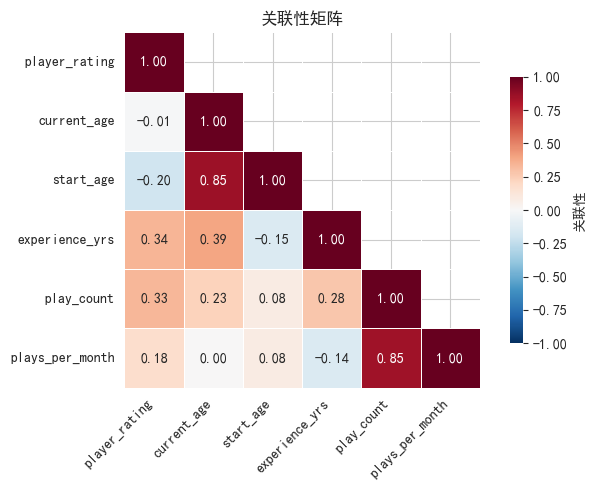
\includegraphics[width=0.6\textwidth]{correlation_matrix.png}
	\caption{核心变量相关性矩阵}
	\label{fig:corr}
\end{figure}

从图中可以看出:  
\begin{itemize}
	\item \textbf{起步年龄(start\_age)} 与当前评分(player\_rating)呈中等负相关($r\approx-0.20$),提示“越早入门→越高分数”的初步趋势。  
	\item \textbf{累计游玩年数(experience\_yrs)} 与评分呈正相关($r\approx0.34$),而每月游玩次数(plays\_per\_month)与评分的相关性稍弱($r\approx0.18$),表明总投入量比频率投入更能解释分数差异。  
	\item \textbf{起步年龄} 与当前年龄高度相关($r\approx0.85$),符合二者计算逻辑;其他变量之间相关度均在可接受范围内,无严重多重共线问题。  
\end{itemize}

本节结果既为后续回归模型中变量筛选提供了直观依据,也为“年龄天赋”与练习量对评分的相对重要性提供了初步定量支持。

\subsection{入坑年龄与玩家 Rating 的关系}

图~\ref{fig:age_loess} 给出了玩家 Rating 与“入坑年龄”之间的局部加权平滑曲线(LOESS, $\mathrm{frac}=0.35$),并用浅黄、浅橙、浅粉三色背景区分了三个阶段:12–15 岁、15–18 岁、18–24 岁。总体来看,随着入坑年龄推后,玩家 Rating 呈缓慢下降趋势,且在 15–18 岁区间波动最为平缓。

\begin{figure}[htbp]
	\centering
	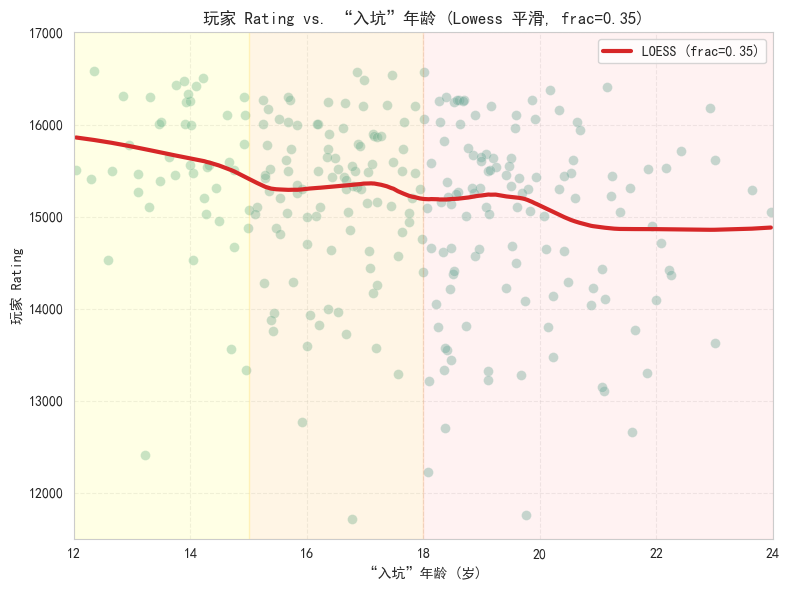
\includegraphics[width=0.6\textwidth]{fig2.png}
	\caption{玩家 Rating vs.\ “入坑”年龄 (Lowess 平滑, $\mathrm{frac}=0.35$)}
	\label{fig:age_loess}
\end{figure}

图~\ref{fig:age_playcount} 将玩家按累计游玩次数分为六级(≤500、501–1000、1001–1500、1501–2000、2001–2500、>2500),并叠加 OLS 线性拟合(虚线)。可以看出:  
\begin{itemize}
	\item \textbf{高投入带来高分:} 游玩次数越多(颜色由红至紫渐深),总体分布越靠上,说明练习量对 Rating 有显著拉动作用;  
	\item \textbf{年龄效应依旧显著:} 即便剔除练习量差异,OLS 拟合斜率仍为负,表明入坑越早的玩家更容易达到更高水平;  
	\item \textbf{分级差异明显:} 低投入组(≤500 次)集中在 12\,500–15\,000 区间,中投入组(1\,001–2\,000 次)则上移至 14\,000–16\,000,而最高投入组(>2\,500 次)中不乏超过 16\,500 的高分玩家。
\end{itemize}

\begin{figure}[htbp]
	\centering
	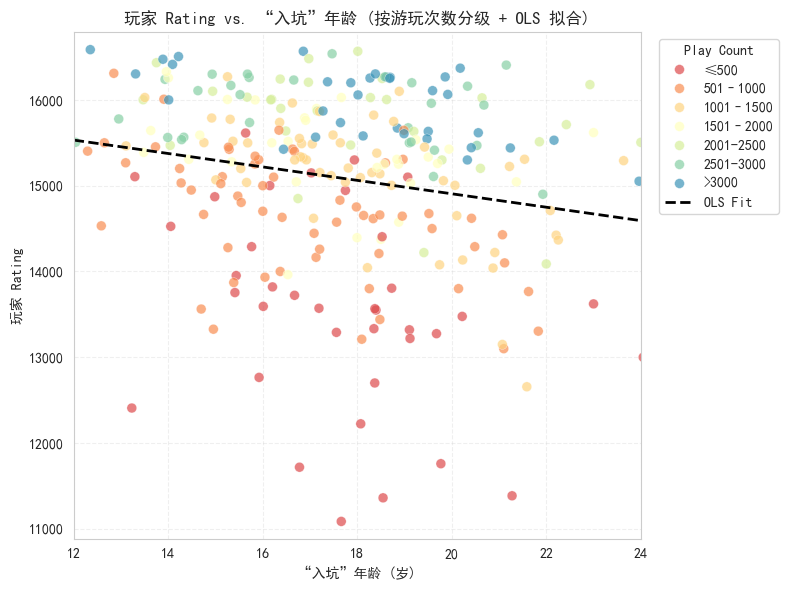
\includegraphics[width=0.6\textwidth]{fig3.png}
	\caption{玩家 Rating vs.\ “入坑”年龄 (按游玩次数分级 + OLS 拟合)}
	\label{fig:age_playcount}
\end{figure}

\subsection{图像结果解读}

\paragraph{图~\ref{fig:age_loess}(LOESS 平滑曲线)}  
该图基于 276 名样本玩家,展示了入坑年龄对最终 Rating 的非线性影响。关键观察有:  
\begin{itemize}
	\item \textbf{整体下降趋势}:从 12 岁到 24 岁,Rating 随入坑年龄呈整体下降,验证“越早入门→越高上限”假说;  
	\item \textbf{15–18 岁平缓期}:在 15–18 岁区间曲线最为平坦,说明这一阶段入门的玩家经过相似年限练习后,水平差异最小;  
	\item \textbf{局部回弹}:15–16 岁出现轻微回升,可能是该年龄段正处于生理与心理的最佳平衡期——既具有足够体力,也保持高注意力;另外18-19 岁左右的微升则可能源于大学新生学业相对宽松,有更多时间专注游戏。  
\end{itemize}

\paragraph{图~\ref{fig:age_playcount}(按游玩次数分级 + OLS 拟合)}  
本图在展示年龄效应的同时,加入练习量控制以剔除其混淆影响:  
\begin{itemize}
	\item \textbf{练习量主效应}:高投入玩家集中在更高分段,说明总体练习量是提升 Rating 的首要因素;  
	\item \textbf{独立年龄效应}:在不同色级分组中,虚线斜率依旧为负,证明年龄效应在练习量相同的前提下仍显著;  
\end{itemize}

\noindent 综上,两张图相辅相成:LOESS 曲线揭示了年龄与表现的非线性关系及特定年龄段的回弹现象;分级散点则在剔除练习量影响后,强化了年龄天赋独立作用的证据。


\newpage

\section{游玩时长与玩家 Rating 的关系}

图~\ref{fig:playtime_saturate} 将样本点按照入坑年龄段(12–15 岁、15–18 岁、18–24 岁)用不同颜色标识,并叠加了指数饱和拟合曲线,可以直观地看到:  游玩 0–2 年内,Rating 从约 12\,500 分迅速提升至约 15\,500 分,边际收益显著。约在 2 年时达到拐点(虚线标注),之后曲线趋于平缓,说明额外投入效用递减。三种入坑年龄段的玩家在前期都表现出相似的上升趋势,但中后期高龄组略显集中在低分区间,提示年龄与练习年限共同影响最终表现。  


\begin{figure}[htbp]
	\centering
	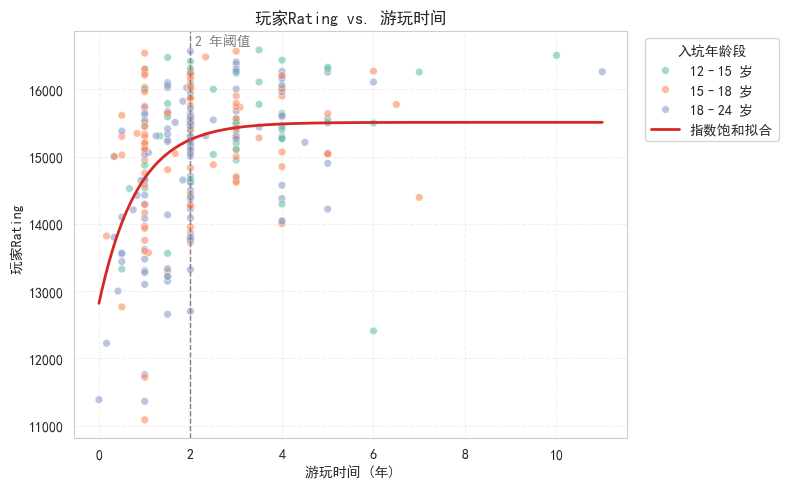
\includegraphics[width=0.65\textwidth]{fig4.png}
	\caption{玩家 Rating vs.\ 游玩时长(按入坑年龄分色 + 指数饱和拟合)}
	\label{fig:playtime_saturate}
\end{figure}

图~\ref{fig:playtime_log} 对游玩时长取 $\log_{10}(\mathrm{years}+1)$ 后作散点和线性回归,进一步凸显了前期投入的高效益:  
\begin{itemize}
	\item \textbf{对数坐标放大前期斜率}:横轴对数化后,0–2 年的点被拉开,线性拟合斜率在此区间更陡,强调早期练习效果;  
	\item \textbf{整体正相关}:尽管后期边际收益递减,对数线性拟合仍然呈显著上升,说明持续投入对提升 Rating 依旧有正向作用。  
\end{itemize}

\begin{figure}[htbp]
	\centering
	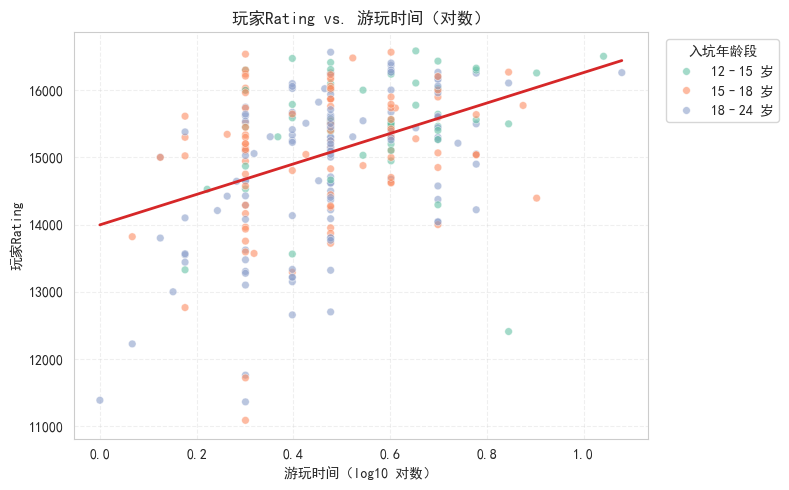
\includegraphics[width=0.65\textwidth]{fig5.png}
	\caption{玩家 Rating vs.\ 游玩时长($\log_{10}$ 对数坐标 + 线性拟合)}
	\label{fig:playtime_log}
\end{figure}

\newpage

\section{回归分析}

本节通过逐步构建 OLS 回归模型,量化练习量与年龄变量对玩家 Rating 的独立与交互效应。

\subsection{基准模型(M0)}
首先构建基准模型,仅纳入练习投入:
\[
\text{player\_rating}_i = \beta_0 + \beta_1\,\text{play\_time\_month}_i
+ \beta_2\,\text{play\_count}_i + \varepsilon_i.
\]
模型结果见表~\ref{tab:m0},$R^2=0.172$,说明游玩时长与总次数共可解释约17.2\% 的评分差异。两项投入系数均高度显著:
\[
\hat\beta_1=14.95\,(p<0.001),\quad
\hat\beta_2=0.0908\,(p<0.001),
\]
意味着每增加一个月游玩时长,平均 Rating (注意是平均Rating,而非实际Rating) 提升约15 分;每增加一次游玩次数,平均提升约0.09 分。

\begin{table}[htbp]
	\centering
	\caption{基准模型 M0 回归结果}\label{tab:m0}
	\begin{tabular}{lcc}
		\toprule
		& Coef.      & $p$-value  \\\midrule
		Intercept       & $1.450\times10^4$ & $<0.001$ \\
		play\_time\_month & $14.95$     & $<0.001$ \\
		play\_count       & $0.0908$    & $<0.001$ \\
		\midrule
		$R^2$           & \multicolumn{2}{c}{0.172} \\
		Adj.\,$R^2$     & \multicolumn{2}{c}{0.166} \\
		\bottomrule
	\end{tabular}
\end{table}

\subsection{加入年龄变量(M1)}
在 M0 基础上,增加当前年龄 \(\text{current\_age}\) 与起步年龄 \(\text{start\_age}\) 两项:
\[
\text{player\_rating}_i =
\]
\[
\beta_0
+ \beta_1\,\text{play\_time\_month}_i
+ \beta_2\,\text{play\_count}_i \\
+ \beta_3\,\text{current\_age}_i
+ \beta_4\,\text{start\_age}_i
+ \varepsilon_i.
\]
F 检验表明与 M0 相比增量显著($F=12.25$, $p=5.4\times10^{-4}$),$\Delta R^2=0.036$,模型解释力提升至 20.8\%。主要系数如下(详见表~\ref{tab:m1}):
\[
\hat\beta_3=-36.50\;(p=0.001),\quad
\hat\beta_4=-37.83\;(p<0.001),
\]
表明在控制练习量后,当前年龄和起步年龄每增加 1 岁,平均Rating降低约 36–38 分,进一步支持“早起步”假说。

\begin{table}[htbp]
	\centering
	\caption{模型 M1 回归结果(含年龄变量)}\label{tab:m1}
	\begin{tabular}{lcc}
		\toprule
		& Coef.      & $p$-value  \\\midrule
		Intercept       & $1.585\times10^4$ & $<0.001$ \\
		play\_time\_month & $15.97$     & $<0.001$ \\
		play\_count       & $0.1003$    & $<0.001$ \\
		current\_age      & $-36.50$    & $0.001$  \\
		start\_age        & $-37.83$    & $<0.001$ \\
		\midrule
		$R^2$           & \multicolumn{2}{c}{0.208} \\
		Adj.\,$R^2$     & \multicolumn{2}{c}{0.199} \\
		$\Delta R^2$    & \multicolumn{2}{c}{0.036} \\
		\bottomrule
	\end{tabular}
\end{table}

\paragraph{多重共线性}  
注意到 \(\text{current\_age}\) 与 \(\text{start\_age}\) 高度相关,模型的条件数很大,提示存在较强多重共线性。但两者系数方向一致,且统计显著,说明二者均能捕捉到年龄对评分的负向影响。

\subsection{交互效应模型(M2)}
最后在 M1 中加入“起步年龄 × 总投入次数”交互项,以检验“早起步”是否增强练习收益:
\[
\begin{aligned}
	\text{player\_rating}_i =\;&\beta_0
	+ \beta_1\,\text{play\_time\_month}_i \\
	& + \beta_2\,\text{play\_count}_i
	+ \beta_3\,\text{current\_age}_i
	+ \beta_4\,\text{start\_age}_i \\
	&+ \beta_5\,(\text{start\_age}_i \times \text{play\_count}_i)
	+ \varepsilon_i.
\end{aligned}
\]
交互项系数 \(\hat\beta_5=-0.0426\;(p=0.002)\),显著为负,表明当起步年龄越高时,每增加一次游玩次数带来的评分增益越小,即“早起步”的玩家不仅基线更高,且练习效率更优(表~\ref{tab:m2})。

\begin{table}[htbp]
	\centering
	\caption{交互模型 M2 回归结果}\label{tab:m2}
	\begin{tabular}{lcc}
		\toprule
		& Coef.      & $p$-value  \\\midrule
		Intercept             & $1.454\times10^4$ & $<0.001$ \\
		play\_time\_month       & $11.43$     & $0.001$  \\
		play\_count             & $0.9108$    & $<0.001$ \\
		current\_age            & $-0.743$    & $0.962$  \\
		start\_age              & $-1.696$    & $0.913$  \\
		start\_age:play\_count  & $-0.0426$   & $0.002$  \\
		\midrule
		$R^2$                 & \multicolumn{2}{c}{0.236} \\
		Adj.\,$R^2$           & \multicolumn{2}{c}{0.225} \\
		\bottomrule
	\end{tabular}
\end{table}

\noindent\emph{小结}:  
\begin{itemize}
	\item 基准模型确认了练习量对 Rating 的显著正效应;  
	\item 加入年龄变量后,起步年龄和当前年龄对评分均有显著负效应,$\Delta R^2=0.036$;  
	\item 交互分析表明,“起步年龄”还能调节练习收益,进一步佐证“年龄天赋”在音游表现中的重要作用。  
\end{itemize}

\section{随机森林特征重要度}

为了补充 OLS 回归的线性假设,本研究进一步使用随机森林回归对玩家 Rating 进行预测,并评估各特征的重要度。输入变量包括累计游玩月份(\(\text{play\_time\_month}\))、总游玩次数(\(\text{play\_count}\))、当前年龄(\(\text{current\_age}\))、起步年龄(\(\text{start\_age}\))、月均游玩次数(\(\text{plays\_per\_month}\))与年均游玩次数(\(\text{plays\_per\_year}\))。模型采用 500 棵树的随机森林,5 折交叉验证下平均 \(R^2=0.591\),表明非线性模型对 Rating 的解释力远超线性回归。

\begin{table}[htbp]
	\centering
	\caption{随机森林特征重要度}\label{tab:rf_importance}
	\begin{tabular}{lcc}
		\toprule
		特征               & 相对重要度 & 排名 \\\midrule
		play\_count       & 0.719  & 1 \\
		start\_age        & 0.110  & 2 \\
		current\_age      & 0.072  & 3 \\
		plays\_per\_month & 0.036  & 4 \\
		plays\_per\_year  & 0.036  & 5 \\
		play\_time\_month & 0.027  & 6 \\
		\bottomrule
	\end{tabular}
\end{table}

从表~\ref{tab:rf_importance} 可见,\textbf{总游玩次数(play\_count)}以 71.9\% 的相对重要度遥遥领先,凸显了投入量对最终表现的主导作用;其次是\textbf{起步年龄(start\_age)}与\textbf{当前年龄(current\_age)},合计占比约 18\%,验证了年龄因素在控制练习量后仍具有显著影响;\textbf{月/年均游玩频率} 和 \textbf{累计时长} 的重要度较低。该结果进一步支持:  
\begin{itemize}
	\item 练习量(尤其是总次数)是提高 Rating 的关键驱动;  
	\item 年龄相关变量在非线性框架中仍贡献明显,且排名仅次于练习量;  
	\item 频率指标与时长在总体模型中的解释力相对有限(省流:虽然总体PC越多分越高,但是并没有“推越多打越好”)。  
\end{itemize}

综合 OLS 与随机森林分析,可得结论:\emph{练习量}是决定音游水平的首要因素,而\emph{年龄天赋}(起步年龄与当前年龄)在去除练习量影响后依然对表现有中等效应,且二者在非线性模型中保持稳定的重要度排序。

\subsection{主观天赋认知与实际表现}

图~\ref{fig:belief_box} 展示了根据玩家对“年龄天赋”重要性的主观认知(Question1)将样本分为“重要”、“不重要”与“存在但不重要”三组后,其 Rating 分布的箱型图。可以看到:
\begin{itemize}
	\item 各组的中位数相近,大约位于 15\,000–15\,300 分之间,说明玩家的主观认知与其实际分数水平并无显著差异;  
	\item “重要”组的中位数略高于“不重要”组,但与“存在但不重要”组相比差异不大;  
	\item 三组的四分位距(IQR)和离群点分布也大致相当,进一步表明主观评价并不能有效预测玩家的实际表现。
\end{itemize}

\begin{figure}[htbp]
	\centering
	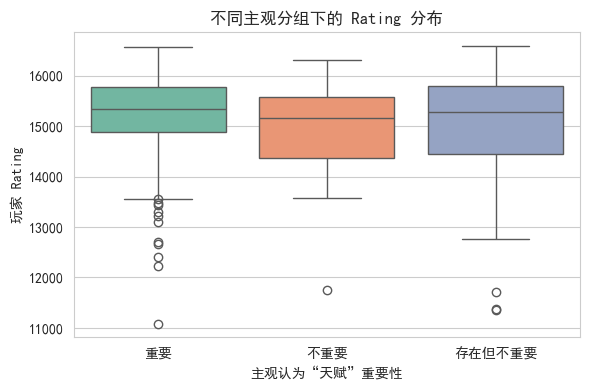
\includegraphics[width=0.7\textwidth]{fig6.png}
	\caption{不同主观分组下的玩家 Rating 分布}
	\label{fig:belief_box}
\end{figure}

	
	\bibliographystyle{unsrt}
	\begin{thebibliography}{9}
		\bibitem{bartholow2014reaction}
		Bartholow, B. et al. Reaction Time and Skill Acquisition in Youth Sports. \emph{J.~Sports Sci.}, 2014.
		
		\bibitem{dodonova2022esports}
		Dodonova, Y. Age-Related Performance Curves in Professional Esports. \emph{Frontiers in Psychology}, 2022.
		
		\bibitem{Watanabe2007}
		Watanabe D., Savion-Lemieux T., Penhune V.\hspace{0pt}B. (2007).
		The effect of early musical training on bimanual coordination and timing.
		\emph{Brain and Cognition}, 64(2), 152–163.
		
		\bibitem{Bailey2013}
		Bailey J.\hspace{0pt}A., Penhune V.\hspace{0pt}B. (2013).
		A sensitive period for musical training: Contributions of age of onset and cognitive abilities.
		\emph{Annals of the New York Academy of Sciences}, 1252, 163–170.
		
		\bibitem{Thompson2014}
		Thompson J.\hspace{0pt}J., Blair M.\hspace{0pt}R., Henrey A.\hspace{0pt}J. (2014).
		Over the hill at 24: Persistent age-related cognitive-motor decline in reaction times in an action video game.
		\emph{PLOS ONE}, 9(4), e94215.
		
		\bibitem{Ericsson1993}
		Ericsson K.\hspace{0pt}A., Krampe R.\hspace{0pt}T., Tesch-R{\"o}mer C. (1993).
		The role of deliberate practice in the acquisition of expert performance.
		\emph{Psychological Review}, 100(3), 363–406.
		
		\bibitem{Macnamara2014}
		Macnamara B.\hspace{0pt}N., Hambrick D.\hspace{0pt}Z., Oswald F.\hspace{0pt}L. (2014).
		Deliberate practice and performance in music, games, sports, education, and professions: A meta-analysis.
		\emph{Psychological Science}, 25(8), 1608–1618.
		
		\bibitem{Gullich2017}
		G{\"u}llich A. (2017).
		International medallists’ and non-medallists’ developmental sport activities–a matched-pairs analysis.
		\emph{Journal of Sports Sciences}, 35(23), 2281–2288.
		
		\bibitem{Vaeyens2009}
		Vaeyens R., Lenoir M., Williams A.\hspace{0pt}M., Philippaerts R.\hspace{0pt}M. (2009).
		Talent identification and development programmes in sport: Current models and future directions.
		\emph{Sports Medicine}, 39(9), 703–714.
	\end{thebibliography}
	
\end{document}
